\cotefile{157-2}
\scanpage{398}\mspage{137}
12. Retour sur les ``catégories de chemins'' \deleted{\unsure{d}}dans $\mathrm{Cat}$, comme
catégorie de modèles pour $\mathrm{Hot}$.

Je \unsure{vois|vais} \unsure{actuellement} deux applications intéressantes
du formalisme des chemins dans les catégories.
L'une, qui m'a surtout forcé la main, est
pour pouvoir construire des $\mathrm{Hom}\,\mathrm{cat}$, \uline{$\mathrm{Hom}$
externes} à valeurs dans $\mathrm{Hot}$, pour tout \inserted{pré}dérivateur
$\mathbb D$ défini par un couple $(M,\Sigma)$ (et je
ne connais pas \unsure{de|des} prédérivateur qui ne
soit défini ainsi.

L'autre application est pour avoir dans $(\mathrm{Cat}$,
une \uline{construction} \uline{fonctorielle}, en termes
d'un objet $X$ quelconque ou d'une \deleted{\unsure{$f\colon Y$|$f\colon X$}}
flèche $X\unsure{\text{---}|\longrightarrow}Y$, de l'analogue du formalisme
de Cartan-Serre sur les espaces de
chemins. Dans ce cadre, il est entendu
qu'on prend toujours $\Sigma_X=\mathrm{Fl}(X)$, ensemble de
\uline{toutes} les flèches de $X$. Pour construire
fonctoriellement en $X$ de $(\mathrm{Cat})$
\diagram{\begin{tikzcd}[ampersand replacement=\&]
\underline{\mathrm{Ch}}_{\infty}(X) \arrow[d] \\
X\times X
\end{tikzcd}}
il faut avoir fixé un syst. projectif
\[
\underline t=(t_n)_{\unsure{n\in\mathbb N|\in\mathbb N}}
\]
% archive sheet number: 397
\scanpage{399}\mspage{138}
de $\unsure{\underline{\mathrm{Ty}}|\underline{\mathrm{Tz}}}$ qui soit cofinal dans $\underline{\mathrm{Ty}}$, ce qui signifie
simplement que parmi les $t_n$ il y en a de longueur
utile arbitrairement grande (et comme
\[
n\unsure{\mathrel{\vdash\!\dashv}|\longmapsto}\operatorname{long.ut.}(t_n)
\]
est croissante, cela implique que $\operatorname{long.ut.}(t_n)$
tend vers $+\infty$ pour $n\longrightarrow+\infty$). \deleted{\illegible{1}} Les
faits principaux à vérifier \inserted{ensuite} (si faire se peut)
sont les propriétés \unsure{essentielles} des flèches
dans le diagramme
\diagram{\begin{tikzcd}[ampersand replacement=\&,column sep=small]
\& X \arrow[d,"\tau"] \& \& \\
\& \underline{\mathrm{Ch}}_{\infty}(X)
  \arrow[d,"{\deleted{\unsure{\varphi}}p}"]
  \arrow[ddl,bend right=20,"\sigma"'] \arrow[ddr,bend left=20,"{\beta}",-{Circle[length=1.4pt]}] \& \& \\
\& X\times X \arrow[dl,"\mathrm{pr}_1"'] \arrow[dr,"\mathrm{pr}_2"]
 \& \& \left|\begin{aligned}\sigma\tau&=\beta\deleted{\unsure{\tau}}\tau=\mathrm{id}_X\\
 \unsure{p|\varphi}\tau&=\mathrm{diag}_X\end{aligned}\right.\\
X \& \& X\mathpunct{,} \&
\end{tikzcd}}
et plus généralement, pour une flèche \deleted{\unsure{$X'\longrightarrow X$}}
\[
X'\xrightarrow{f}X
\]
dans $\mathrm{Cat}$, \deleted{\unsure{des}} des flèches dans le diagramme
correspondant
\diagram{\begin{tikzcd}[ampersand replacement=\&,column sep=small]
\& \overline{X'}=\mathrm C(f) \arrow[ddl] \arrow[dr,"g"] \arrow[ddrr,bend left=22,"\bar f"] \& \& \& \bar f\unsure{\alpha|\alpha'}=(\beta g)\alpha=f\\
\& \& \deleted{\unsure{X}}\mathrm{Ch}_{\infty}(X) \arrow[ddl,"\sigma" description] \arrow[dr,"\beta"] \& \& \\
X' \arrow[uur,dashed,bend left=30,"\alpha"] \arrow[dr,"f"'] \& |[draw,ellipse,inner sep=1pt]| \text{cart} \& \& X \& \\
\& X \& \& \&
\end{tikzcd}}
et plus particulièrement de $\beta g$. La flèche
% archive sheet number: 398
\scanpage{400}\mspage{139}
en pointillés $\alpha$ est la section de $\overline{X'}$ sur $X'$
déduite de la section $\tau$ de $\mathrm{Ch}_{\infty}(X)$ sur $X$,
qui réalise la décomposition de $f$ en
\[
X'\xrightarrow{\alpha}\overline{X'}\xrightarrow{\bar f}X
\]
où $\bar f$ devrait être une flèche ``\uline{fibrante}'' et
une $\mathrm{Hot}$-équivalence, $\alpha$ une flèche ``\uline{cofibrante}''
au sens de Thomason. (\deleted{\unsure{M}}Mais s'il en est ainsi,
est à voir !) Voici pour le moment les
propriétés essentielles que je voudrais vérifier.

$1^\circ$) $p$ est lisse et propre, et \inserted{est} une $\mathrm{HOT}$-fibration. \deleted{\unsure{De}}

$2^\circ$) Donc il en est de même de $\sigma=\mathrm{pr}_1p$ et $\beta=\mathrm{pr}_2p$.
De plus, ce sont des $\mathrm{HOT}$-fibrations \uline{triviales}, i.e.
à fibres \deleted{\unsure{contractiles}} \inserted{asphériques}.

$3^\circ$) Plus généralement \inserted{(pour ce qui concerne $\beta$)}, $\overline{X'}\xrightarrow{\bar f}X$ devrait \inserted{encore} être
propre et lisse et une $\mathrm{HOT}$-fibration, mais bien
sûr \deleted{\unsure{de}} \inserted{en général} pas triviale. (Elle devrait être triviale ssi
$f$ est une $\mathrm{Hot}$-équivalence.)
% slanted
\margin{\unsure{résulte} \unsure{formellement} de $1^\circ$ \deleted{\unsure{et $2^\circ$}} \unsure{et de} \unsure{cf p.|cf p.$^{\circ}$} 170}

Un mot sur la ``dualité''. Les énoncés sur
$\sigma$ (resp. $\beta$) se traduisent en énoncés sur
$\beta$ (resp. $\sigma$) par passage de $\underline t$ à $\underline t^{\circ}=(\deleted{\unsure{p}}t_n^{\circ})$,
où $\unsure{\tau|z}\unsure{\relbar|\longrightarrow}\tau^{\circ}$ est le foncteur de $\unsure{\mathrm{Ty}|\mathrm{Tz}}$ ``passage
à \deleted{\unsure{au dual}} l'intervalle opposé''. \unsure{On a|Oui|Or}, en effet
% archive sheet number: 399
\scanpage{401}\mspage{140}
un isom fonctoriel en $X$ (passage au chemin
opposé)
\[
\begin{tikzpicture}[baseline=(f.base)]
\node[inner sep=3pt] (f) {$\mathrm{Ch}_{\infty}^{\underline t}(X)\xrightarrow{c\unsure{\mathrel{\vdash\!\dashv}|\mapsto}c^{\circ}}\underline{\mathrm{Ch}}_{\infty}^{\underline t^{\circ}}(X)$};
\draw (f.north west)--(f.south west)--(f.south east)--(f.north east);
\end{tikzpicture}
\]
% slanted
\margin{cf page 143 pour le passage de $\underline t$ à $\underline t^{-}$}
qui ``échange source et but''. Bien sûr, on
a intérêt à prendre $\unsure{\underline{\bar t}|\underline t}$ tel qu'on ait
$\underline t=\underline t^{\circ}$ (c'est ce que j'avais fait, par un
\unsure{sûr|sain} instinct, dès le début de $\overline{\underline{\mathrm V}}$), de
sorte qu'on a \unsure{un|une} \inserted{foncteur} involutif canonique
\[
\underline{\mathrm{Ch}}_{\infty}(X)\xrightarrow{c\mathrel{\vdash\!\dashv}c^{\circ}}\underline{\mathrm{Ch}}_{\infty}(X)
\]
(je laisse tomber à nouveau l'exposant $\underline t$),
qui ``échange source et but''. Donc on trouve,
à isom. \inserted{can.} près, la ``$=$'' factorisation de $f\colon X'\unsure{\relbar|\to}X$
en $\bar f\circ\alpha$, \deleted{\unsure{que}} si on fait comme \unsure{dessus} page
38, pour définir $\overline{X'}$ et $\alpha$, ou si dans ce
diagramme on intervertit les rôles de $\sigma$ et
de $\beta$.

Enfin

$4^\circ$) Si
\[
c\colon \unsure{a|\bullet}\longrightarrow b
\]
est un chemin quelconque dans $X$, on
% slanted
\margin{\unsure{Surtout} pour se borner au cas où $c$ serait un des $t_n$ !}
voudrait en conclure une \unsure{iso.} dans
$\mathrm{Hot}$ (de ``transport par $c$'')
\[
\overline{X'}_a\xrightarrow{\substack{\bar c\\[-2pt]\sim}}\overline{X'}_b,
\]
% slanted
\margin{décrire quand même l'effet sur les $\pi_0$ !}
avec bien sûr transitivité pour la composition,
% archive sheet number: 400
\scanpage{402}\mspage{141}
ce qui donnera aussi
\[
\overline{c^{\mathrm{opp}}}=\bar c^{-1}
\]
(en admettant que les chemins triviaux $a\overset{\mathrm{id}}{\unsure{\dashv|\to}}a$
donnent l'identité $\overline{X'}_a\overset{\substack{\mathrm{id}\\[-2pt]\sim}}{\relbar}X'_a$ !]. \deleted{\unsure{En d'autre}}

Bien sûr, $\bar c$ ne doit dépendre que de la
\uline{classe d'homotopie} de $\bar c$ (dans $\underline{\mathrm{Ch}\deleted{\unsure{\mathrm{loc}}}}_{\tau}(X;a,b)$ \deleted{\unsure{ou}}
\deleted{\unsure{ou mieux,}} \inserted{ou même} \deleted{dans} $C=\underline{\unsure{\mathrm{Ch}|\mathrm{ChP}}}(X,a,b)$, catégorie de
tous les chemins dans $X$, de $a$ vers $b$, de
type non précisé). En d'autres termes, on
doit avoir un foncteur
\[
\begin{aligned}
\Pi(X)&\longrightarrow\mathrm{Hot}\\
a&\unsure{\mathrel{\vdash\!\dashv}|\longmapsto}\mathrm{hot}(\overline{X'}_a)
\end{aligned}
\]
du groupoïde fondamental de $X$ dans $\mathrm{Hot}$.
\deleted{\unsure{Et on aura}} À vrai dire, ceci n'a rien à
voir avec la situation particulière étudiée
ici, -- ça \deleted{\unsure{dev}}doit marcher chaque fois qu'on
a une $\mathrm{HOT}$-fibration, ici $\overline{X'}\longrightarrow X$,
% slanted
\margin{Ici aussi, il faudrait décrire l'effet du transport $\bar c$ sur le $\unsure{\bar\pi_0|\pi_0}$ des fibres.}
mais aussi $\underline{\mathrm{Ch}}_{\infty}(X)\longrightarrow X\times X$\textsuperscript{*}. Et
pour une $\mathbb D$-fibration \inserted{$X'\to X$} ($\mathbb D$ un dérivateur
quelconque), \inserted{et $a\in\mathbb D(e)$,} on doit avoir de $=$ deux foncteurs
\[
\Pi(X)\rightrightarrows\mathbb D(e)
\]
correspondants à
\[
\left\{\begin{aligned}
x&\longmapsto H^{\bullet}_{\mathbb D}(X'_{\unsure{x|*}},a)\\
\unsure{x|\lambda}&\unsure{\mapstochar\relbar|\mapsto}H^{\mathbb D}_{\bullet}(X'_x,a)
\end{aligned}\right.
\]
% archive sheet number: 401
\scanpage{403}\mspage{142}
Le cas qui nous occupe ici serait celui où
$\mathbb D=\mathrm{HOT}$, et on prend $H^{\mathbb D}_{\bullet}$, et $a={}$objet final de
$\mathbb D(e)=\mathrm{Hot}$.)

$5^\circ$) Si $1^\circ,2^\circ,3^\circ$ sont vérifiés, on est moralement
sûr que la construction de $\underline{\mathrm{Ch}}_{\infty}(X)$ est bel
et bien l'équivalent exact du formalisme de
Cartan-Serre. Pour en avoir le cœur totalement
\unsure{net}, i.e. raccrocher \inserted{explicitement} cette théorie aux
constructions classiques, il faudrait \deleted{\unsure{poser}} prouver un
\uline{énoncé de comparaison} avec la théorie
semisimpliciale, qui dirait essentiellement
ceci : Si on désigne, pour $X$ dans $\mathrm{Cat}$, par
$\widetilde X$ l'objet associé de $\mathbb{\Delta}^{\wedge}$ (le ``nerf'' de $X$),
alors la flèche
\diagram{\begin{tikzcd}[ampersand replacement=\&,row sep=tiny]
\widetilde{\underline{\mathrm{Ch}}_{\infty}(X)} \arrow[r] \& \widetilde{X\times X} \arrow[d,phantom,sloped,"\simeq" description]\\
\&\widetilde X\times\widetilde X
\end{tikzcd}}
\deleted{est \unsure{transformée}} dans $\mathbb{\Delta}^{\wedge}/\widetilde{X\times X}$, est
$W$-équivalente sur $\widetilde{X\times X}$ à la flèche
\[
\mathrm{Ch}(\widetilde X)\longrightarrow\widetilde X\times\widetilde{\unsure{X|Y}}
\]
de la théorie \unsure{ssimpliciale|simpliciale|semisimpliciale} des chemins (à
supposer qu'il y ait une telle flèche classique,
définie pour \uline{tout} objet $X$ de $\mathbb{\Delta}^{\wedge}$). Ou
qu'on ait \inserted{tout au moins} des isom. canoniques \inserted{dans} $\mathrm{Hot}$
\[
\mathrm{hot}_{\mathrm{Cat}}\bigl(\underline{\mathrm{Ch}}_{\infty}(X;a,b)\bigr)
\simeq\mathrm{hot}_{\mathbb{\Delta}^{\wedge}}\bigl(\mathrm{Ch}(\widetilde X;\tilde a,\tilde b)\bigr).
\]
% archive sheet number: 402
\scanpage{404}\mspage{\deleted{\unsure{14}}143}
Dans $1^\circ$ et $3^\circ$, on veut prouver que certaines flèches
\inserted{($p$ et $\bar f$)} sont à la fois \uline{propres} et \uline{lisses} -- ce qui est vraiment
\unsure{idéal|idiot} ! Je dis qu'il suffit à chaque fois de
prouver l'un des deux, que l'autre s'en déduit
(comme ``cas particulier'') par dualité. Pour ceci,
notons
\[
\tau\unsure{\mapstochar\relbar|\mapsto}\tau^{-}
\]
l'automorphisme (\uline{pas} \uline{anti}-automorphisme) de
$\unsure{\underline{\mathrm{Ty}}|\underline{\mathrm{Tz}}}$ qui consiste à changer de \unsure{signe|signes} toutes les
flèches de transition -- c'est donc, \inserted{au niveau des objets,} l'unique
autom. du monoïde libre $\mathrm{Ty}$, qui échange
$\Delta_+$ et $\Delta_-$. Au système projectif $\underline{\unsure{t|f}}$ de $\underline{\mathrm{Ty}}$
correspond le système projectif $\underline t^{-}$. Ceci
dit, on a un isom. de catégories
\[
\boxed{\underline{\mathrm{Ch}}_{\infty}^{\underline t}(X^{\circ})
\simeq\bigl(\underline{\mathrm{Ch}}_{\infty}^{\underline t^{-}}(X)\bigr)^{\circ}}
\]
% slanted
\margin{cf page 140 pour le passage de $\underline t$ à $\underline t^{\circ}$}
et \deleted{le foncteur} le diagramme commutatif
\diagram{\begin{tikzcd}[ampersand replacement=\&,row sep=large]
\underline{\mathrm{Ch}}_{\infty}^{\underline t}(X^{\circ}) \arrow[d,"p^{\underline t}_{X^{\circ}}"] \& \simeq \& \underline{\mathrm{Ch}}_{\infty}^{\underline t^{-}}(X)^{\circ}\arrow[d,"{(p_X^{\underline t^{-}})^{\circ}}"]\\
\deleted{\unsure{C}}X^{\circ}\times X^{\circ} \& = \& (X\times X)^{\circ}
\end{tikzcd}}
Ainsi, dire que $p^{\underline t}_X$ est lisse, i.e que
$(p^{\underline t}_X)^{\circ}$ est propre, équivaut à dire que $p^{\underline t}_{X^{\circ}}$ est
propre.
% archive sheet number: 403
\scanpage{405}\mspage{144}
Il nous reste donc, à ce sujet, que deux faits à
vérifier : la lissité de $p\colon\underline{\mathrm{Ch}}_{\infty}(X)\unsure{\relbar|\to}X\times X$,
et celle de $\bar f\colon\overline X\longrightarrow X$.

a) lissité de $p\colon\inserted{\underline{\mathrm{Ch}}_{\infty}(X)\to X\times X}$ On se donne une flèche
\[
w\colon(a,b)\longrightarrow(a',b')\qquad
\text{i.e. }\begin{aligned}u&\colon a\to a'\\v&\colon b\to b'\end{aligned}
\]
sur la base, un objet $c'$ au-dessus du but
i.e.
\[
c'\in\mathrm{Ch}_{\infty}(X;a',b'),
\]
et on regarde la catégorie des flèches dans
$\underline{\mathrm{Ch}}_{\infty}(X)$, de but $c'$, qui relèvent $w$,
\diagram{\begin{tikzcd}[ampersand replacement=\&]
\underset{\text{variable}}{c^{\deleted{\unsure{*}}}} \arrow[r,"{\unsure{\varphi|\psi}}"] \arrow[d,no head] \& \underset{\text{fixe}}{c'}\arrow[d,no head]\\
(a,b)\arrow[r,"w"]\&(a',b')
\end{tikzcd}}
i.e. \inserted{la catégorie} des couples \deleted{\unsure{$\varphi$}} $(c,\varphi)$, où
\[
\deleted{\unsure{=}}\left\{\begin{aligned}
&c\in\mathrm{Ch}_{\infty}(X;a,b)\\
&\varphi\colon c\longrightarrow c'\quad(\in\mathrm{Ch}_{\infty}(X,a',b')\\
&\text{une flèche induisant }\begin{aligned}u&\ \text{sur les sources}\\v&\ \text{sur les buts.}\end{aligned}
\end{aligned}\right.
\]
\diagram{\begin{tikzcd}[ampersand replacement=\&,column sep=small,row sep=large]
a\arrow[rrrr,dotted,no head,"c"]\arrow[d]\&{}\arrow[d,dotted]\&{}\arrow[d,dotted]\&{}\arrow[d,dotted]\&b\arrow[d]\\
a'\arrow[rrrr,no head,"c'"]\&{}\&{}\&{}\&b'
\end{tikzcd}}
% archive sheet number: 404
\scanpage{406}\mspage{145}
9.11.90

Pour les questions précédentes, relatives aux flèches
dans le diagramme
\diagram{\begin{tikzcd}[ampersand replacement=\&,row sep=small,column sep=small]
\& X\arrow[d,"{\unsure{i|\tau}}"] \& \\
\& \underline{\mathrm{Ch}}_{\infty}^{\deleted{\unsure{t}}}(X)\arrow[d,"p"]\arrow[ddl,"\sigma"']\arrow[ddr,"\beta",-{Circle[length=1.2pt]}]\&\\
\&X\times X\arrow[dl,"{\unsure{p_1|r_1}}"']\arrow[dr,no head,"p_2"]\&\\
X\&\&\unsure{\bar X|X}
\end{tikzcd}}
% slanted
\margin{\deleted{\unsure{figure}}}
, il faut préciser absolument
la description de $\underline{\mathrm{Ch}}_{\infty}(X)$ \uline{dans
$\mathrm{Cat}$}, donc il faut préciser
le système projectif $\underline t\deleted{\unsure{_{\infty}}}=(t_n)_{n\in\mathbb N}$.
Nous allons prendre en effet
\[
t_n=(\underbrace{\deleted{\unsure{\relbar}}\Delta_+\Delta_-}_{\tau_0})^{2n},
\]
avec les morphismes de
transition décrits par ailleurs
\diagram{\begin{tikzcd}[ampersand replacement=\&,row sep=small]
t_{n+p}\arrow[r,{Bar[width=2pt]}-{Bar[width=2pt]}]\arrow[d,phantom,sloped,"=" description]\&t_n\arrow[d,phantom,sloped,"=" description]\\
\tau_0^{2n+2p}\&\tau_0^{\unsure{n|2n}}
\end{tikzcd}}
étant donné par $\delta_p*\mathrm{id}_{\tau_0^{2n}}*\delta_p$, où $\delta_p\colon\tau_0^p\unsure{\relbar|\to}1$ est
la dégénérescence de $\tau_0^p$. Ainsi, on peut
considérer $\mathrm{Ch}_{\infty}(X)$ comme étant la catégorie
des \deleted{\unsure{entre}} chemins \inserted{bi-}infinis dans $X$
\diagram{\begin{tikzcd}[ampersand replacement=\&,column sep=1.8pt,font=\scriptsize,execute at end picture={
\draw (bl.north) .. controls +(0,.44) and +(-.32,0) .. ($(az.north)+(0,.72)$) .. controls +(.32,-.08) and +(0,.44) .. (br.north);
\node[above] at ($(az.north)+(0,.72)$) {$\underline{\mathrm{Ch}}_2$};
\draw (al.north) .. controls +(0,.27) and +(-.28,-.13) .. ($(az.north)+(0,.40)$) .. controls +(.28,-.13) and +(0,.27) .. (ar.north);
\node[above] at ($(az.north)+(0,.40)$) {$\underline{\mathrm{Ch}}_1$};
\node[above,inner sep=0pt] at (az.north) {$\underset{\downarrow}{\underline{\mathrm{Ch}}_0}$};}]
\cdots\arrow[r]\&a_{-5}\&|[alias=bl]|a_{-4}\arrow[l]\arrow[r]\&a_{-3}\&|[alias=al]|a_{-2}\arrow[l,"u_{-2}"']\arrow[r,"u_{-1}"]\&a_{-1}\&|[alias=az]|a_0\arrow[l,"u_0"']\arrow[r,"u_1"]\&a_1\&|[alias=ar]|a_2\arrow[l,"u_2"']\arrow[r,"u_3"]\&a_3\&|[alias=br]|a_4\arrow[l]\arrow[r]\&a_5\&\cdots\arrow[l]
\end{tikzcd}}
avec les $u_i$ des identités pour $|i|$ assez grand.
La sous-catégorie \deleted{\unsure{$\mathrm{Ch}_{t}$}} (pleine)
\deleted{Nous allons regarder cette catégorie}
\[
\underline{\mathrm{Ch}}^{W}_{t_n}(X)=\underline{\mathrm{Ch}}^{W}_{(\Delta_+\Delta_-)^{2n}}
\]
s'identifie à celle pour laquelle on a
\[
u_i\ \text{une identité pour }i\notin[-2\unsure{i|i'}+1,2i]
\]
i.e. les seuls $u_i$ ``significatifs'' sont les
$4i$ flèches $u_{-2i+1},u_{-2i+2}\ \ldots\ u_{2i}$.

Mais il sera \inserted{plus} commode de regarder $\underline{\mathrm{Ch}}_{\infty}(X)$
comme \deleted{\unsure{la}} limite inductive d'une
% archive sheet number: 405
\scanpage{407}\mspage{146}
famille à deux indices de sous-catégories
pleines
\[
\underline{\mathrm{Ch}}_{n,m}^{\deleted{\unsure{W}}}(X)\qquad n,m\in\mathbb Z,\quad\deleted{\unsure{n\leq m}}
\]
en définissant cette catégorie comme \uline{vide} si $n>m$,
et pour $n\leq m$ comme formée des objets
\diagram{\(\left\{\begin{gathered}
\deleted{\unsure{\biggl\{}}(a_i;u_i)_{i\in\mathbb Z}\in\mathrm{Ch}^W_{n,m}(X)\Longleftrightarrow
\begin{aligned}&u_i\text{ une identité pour}\\& i\notin[n,m-1]\end{aligned}\\[5pt]
\begin{tikzcd}[ampersand replacement=\&,column sep=2pt,font=\scriptsize,execute at end picture={
\draw (an.south) .. controls +(0,-.16) and +(-.18,.15) .. ($(an.south)!.5!(am.south)+(0,-.27)$) .. controls +(.18,.15) and +(0,-.16) .. (am.south);
\node[below,font=\scriptsize,align=center] at ($(an.south)!.5!(am.south)+(0,-.28)$) {``\unsure{portion|partie} utile''\\du chemin};}]
\overset{\mathrm{id}}{\cdots}\&a_{n-1}\arrow[r,no head,"\mathrm{id}"]\&|[alias=an]|a_n\arrow[r,no head,"u_n"]\&a_{n+1}\&\cdots\arrow[r,no head]\&a_{m-1}\arrow[r,no head,"u_{m-1}"]\&|[alias=am]|a_m\arrow[r,no head,"\mathrm{id}"]\&a_{m+1}\&\overset{\mathrm{id}}{\cdots}
\end{tikzcd}
\end{gathered}\right.\)}

Donc pour $n=m$, on trouve la sous-catégorie pleine
isomorphe à $X$, formée des chemins infinis
``totalement dégénérés'' i.e. tels que \uline{toutes} les
$u_i$ soient des identités. (Cette sous-cat. de
$\underline{\mathrm{Ch}}_{\infty}$ ne dépend donc pas du choix de $n=m$.)
\diagram{\begin{tikzcd}[ampersand replacement=\&,row sep=tiny,column sep=small]
{}\arrow[r,"\mathrm{id}"]\&a_{-1}\arrow[d,phantom,sloped,"=" description]\&a_0\arrow[l,"\mathrm{id}"']\arrow[r,"\mathrm{id}"]\arrow[d,phantom,sloped,"=" description]\&a_1\arrow[d,phantom,sloped,"=" description]\&{}\arrow[l,"\mathrm{id}"']\\
\&a\&\unsure{a|c}\&a\&
\end{tikzcd}}
Tous les sommets d'un \deleted{\unsure{même}} \inserted{tel} chemin sont égaux
à un même objet \deleted{\unsure{$a$}} de $X$, et les flèches
de transition entre eux sont identiques.

La structure de $\underline{\mathrm{Ch}}^W_{n,m}(X)\simeq\underline{\mathrm{Ch}}^W_{\tau_{n,m}}(X)$
ne dépend que de la longueur $m-n$ de $\tau_{n,m}$,
et de la \uline{\unsure{parité}} de $n$. Si $n$ est pair,
la direction initiale de $\tau_{n,m}$ est positive,
et
\[
\tau_{n,m}=\underbrace{\Delta_+\Delta_-\ \ldots}_{\substack{m-n\ \text{facteurs}\\\text{en alternance}}}
=\begin{cases}
(\Delta_+\Delta_-)^{\frac{m-n}{2}}&\text{si }m\text{ pair}\\
(\Delta_+\Delta_-)^{\frac{m-n}{2}-1}\Delta_+&\text{si }\inserted{\unsure{m\text{ impair}|\text{en général}}}
\end{cases}
\]
tandis que pour $n$ impair c'est juste l'inverse
% archive sheet number: 406
\scanpage{408}\mspage{147}
\[
\tau_{n,m}=\underbrace{\Delta_-\Delta_+\ \ldots}_{\substack{m-n\ \text{facteurs}\\\text{alternés}}}
=\begin{cases}
(\Delta_-\Delta_+)^{\frac{m-n}{2}}&\text{si }m\text{ impair}\\
(\Delta_-\Delta_+)^{\frac{m-n}{2}-1}\Delta_-&\text{si }m\text{ pair}
\end{cases}
\]
La direction initiale est conforme à la parité
de $n$, i.e. égale à $(-1)^n$, tandis que la direction
\deleted{\unsure{fin}} terminale est opposée à la parité de $m$, i.e. égale
à $(-1)^m$.

Je note \deleted{\unsure{c}} que l'on a $\tau_0=(\tau_0)^{\circ}$ d'où
\[
\underline t\deleted{\unsure{\ne}}\unsure{=|\ne}\underline t^{\circ},\quad\inserted{\text{mais}}\quad\underline t\ne\underline t^{-}
\]
et pourtant on a \deleted{\unsure{des}}\unsure{des} isomorphismes fonctoriels
en $X$
\[
\underline{\mathrm{Ch}}^{\deleted{\unsure{W}}}_{\underline t}(X)\simeq
\underline{\mathrm{Ch}}^{\deleted{W}}_{\underline t^{-}}(X)
\]
respectant source et but, à cause d'un isomorphisme
\[
\underline t\simeq\underline t^{-}\qquad\text{dans }\mathrm{Pro}(\unsure{\underline{\mathrm{Ty}}|\underline{\mathrm{Tz}}})
\]
On peut dire p.ex. que le \uline{foncteur translation} \inserted{$T^{p}_{\deleted{\unsure{p}}}$}
d'amplitude $p$ \inserted{(pour $p\in\mathbb Z$)} est défini sur $\underline{\mathrm{Ch}}^{W}_{\underline t}(X)$, par
\[
\left\{\begin{aligned}
&T^{p}_{\deleted{\unsure{p}}}\bigl(((a_i),(u_i))_{i\in\mathbb Z}\unsure{=}\bigr)=((\deleted{\unsure{a}}b_j,v_j))_{j\in\mathbb Z}\\
&\text{avec }\quad\begin{aligned}b_j&=a_{j-p}\\v_j&=u_{j-p}\end{aligned}
\end{aligned}\right.
\]
et que
\[
\begin{aligned}
T^{p}_{\deleted{\unsure{p}}}\colon&
\left\{\begin{aligned}
\underline{\mathrm{Ch}}^{\deleted{W}}_{t}(X)&\xrightarrow{\sim}\underline{\mathrm{Ch}}^{\deleted{W}}_{-t}(X)\\
\underline{\mathrm{Ch}}^{\deleted{W}}_{-t}(X)&\unsure{\simeq|\xrightarrow{\sim}}\underline{\mathrm{Ch}}^{\deleted{W}}_{t}(X)
\end{aligned}\right\}\ \text{si }p\text{ impair}\\
T^{p}_{\deleted{\unsure{p}}}\colon&
\left\{\begin{aligned}
\underline{\mathrm{Ch}}^{\deleted{W}}_{t}(X)&\xrightarrow{\sim}\underline{\mathrm{Ch}}^{\deleted{W}}_{t}(X)\\
\underline{\mathrm{Ch}}^{\deleted{W}}_{-t}(X)&\simeq\underline{\mathrm{Ch}}^{\deleted{W}}_{-t}(X)
\end{aligned}\right\}\ \text{si }p\text{ pair}
\end{aligned}
\]
% archive sheet number: 407
\scanpage{409}\mspage{148}
\deleted{\unsure{en d'autres}}

En d'autres termes, on peut \unsure{formellmt|formellement} regarder
la catégorie somme
\[
\underline{\mathrm{Ch}}_{\pm}^{\deleted{\unsure{W}}}(X)=
\underline{\mathrm{Ch}}_+^{\deleted{W}}(X)\amalg\underline{\mathrm{Ch}}_-^{\deleted{W}}(X)
\]
et \deleted{\unsure{T}}l'opération translation $T$ comme un
automorphisme qui échange les deux
morceaux, et $T^p$ n'est autre que son
itéré $p$-ième, qui échange les morceaux $+$ et $-$
si $p$ impair, qui les stabilise si $p$ pair.

Il y a aussi l'automorphisme \inserted{involutif} de \deleted{\unsure{symétrie}} \inserted{passage}
au chemin opposé, qui échange source et but,
et que je définis (conformément à l'isom
canonique identique
\[
\underline t\xrightarrow{\sim}\underline t^{\circ}\quad)
\]
comme la symétrie $S$
\[
\left\{\begin{aligned}
&\deleted{\unsure{\mathrm{opp}}}S\bigl((a_i)(u_i)\bigr)=\bigl((b_j),(\unsure{u_j|v_j})\bigr)\qquad\text{avec}\\
&b_j=a_{-j}\\
&u_j\deleted{\unsure{-}}=u_{-j+1}
\end{aligned}\right.
\]
Si je le regarde comme \unsure{opérant} sur $\underline{\mathrm{Ch}}_{\pm}^{W}(X)$,
il est lié \deleted{\unsure{à}}\inserted{a}u foncteur $T$ par
\[
\deleted{\unsure{TS}}\left\{\begin{aligned}S^2&=\mathrm{id}\\STS^{-1}&=T^{-1}\end{aligned}\right.,
\]
de sorte que c'est le groupe $\text{½}$ direct de
$\mathbb Z/2\unsure{\mathbb Z|0}$ par $\mathbb Z$ (groupe affine de dim 1 \unsure{sur}
l'anneau $\mathbb Z$) qui opère sur $\underline{\mathrm{Ch}}_{\pm}$.
% archive sheet number: 408
\scanpage{410}\mspage{149}
On est embarrassé de trouver un automorphisme
$T^2$ de la situation $\underline{\mathrm{Ch}}^{\deleted{\unsure{W}}}_{\infty}(X)\longrightarrow X\times X$, sans qu'il
soit évident que dans $\mathrm{Hot}$, ce foncteur
induise l'identité ! Je ne vois aucun moyen
de relier un chemin $c$ et $T^2c$
par une flèche de $\underline{\mathrm{Ch}}_{\infty}$, ni même par
un chemin ``canonique''. Mais je me dis
que cet automorphisme est \deleted{\unsure{lié}} \inserted{décrit} par un automorphisme,
\deleted{\unsure{du pro}} non pas du système projectif
\[
(\tau_{n,m})_{\substack{n,m\in\mathbb Z^{\circ}\times\mathbb Z\\n\leq m}}
\]
(où \deleted{\unsure{intuitivement}} $\mathbb Z^{\circ}$ désigne l'ens. ordonné
\uline{opposé} de $\mathbb Z$), mais du \uline{pro-objet} de
$\unsure{\underline{\mathrm{Ty}}|\underline{\mathrm{Tz}}}$ qu'il définit (qui est bien sûr ``le $=$''
pour tous les systèmes projectifs cofinaux \inserted{à gauche} dans
$\underline{\mathrm{Ty}}$). Il en résulte déjà que $T^2$
induit l'identité sur l'ind-objet
de $\mathrm{Cat}\,\mathrm{hot}$, $\underline{\underline{\mathrm{Ch}}}_{\infty}^{\deleted{W}}(X)$, et a fortiori sur
l'ind objet correspondant de $\mathrm{Hot}$, ou de
$\mathrm{Hot}_0^{\wedge}$, ou enfin pour l'objet de $\mathrm{Hot}_0^{\wedge}$ lui-même.
\inserted{De $=$ pour les $\underline{\mathrm{Ch}}^{\deleted{W}}_{\infty}(X;a,b)$.} Il s'ensuit, \unsure{revenant} à $\underline{\mathrm{Ch}}^{\deleted{W}}_{\infty}(X)$
lui-même et aux $\underline{\mathrm{Ch}}^{\deleted{W}}_{\infty}(X;a,b)$, que
\deleted{\unsure{les}}l'autom. induit par $T^2$ est \deleted{\unsure{la}}l'identité dans
$\mathrm{Hot}_0^{\wedge}$. J'\unsure{espère} que $\mathrm{Hot}\longrightarrow\mathrm{Hot}_0^{\wedge}$ est
% archive sheet number: 409
\scanpage{411}\mspage{150}
tout au moins fidèle, de sorte que ça prouvera
que $T^2$ induit l'identité dans $\mathrm{Hot}$ également.

Je reviens aux questions $1^\circ$ à $4^\circ$ d'il y a qques
jours. Pour $1^\circ$), il faut prouver que
\[
p\colon\underline{\mathrm{Ch}}^{\deleted{\unsure{W}}}_{\infty}(X)\longrightarrow X\times X
\]
est lisse et propre et une $\mathrm{HOT}$-fibration. Par
dualité, \inserted{$p$} propre résultera de $p$ lisse. Mais
$\underline{\mathrm{Ch}}^{\deleted{W}}_{\infty}(X)$ est $\varinjlim$ des $\underline{\mathrm{Ch}}^{\deleted{W}}_{n,m}(X)$, avec $n\longrightarrow-\infty$, $m\longrightarrow+\infty$,
et où on peut se borner à $n$ et $m$ \uline{pairs}. Or
on voit que pour $n,m$ pairs, \unsure{i.e.|avec} $\tau_{n,m}$ à flèche
initiale \deleted{positive}, directe, à flèche finale rétrograde,
$\underline{\mathrm{Ch}}_{n,m}^{\deleted{W}}(X)\simeq\underline{\mathrm{Ch}}_{\tau_{n,m}}^{\deleted{W}}(X)$ est \inserted{Cat-}\uline{fibrée} sur $X\times X$,
donc \inserted{\deleted{\unsure{une}}}\deleted{$\mathrm{HOT}$-fibration\unsure{,}} lisse (i.e. $\mathrm{HOT}$ lisse),
\unsure{ceci|cela} \unsure{passe} aux $\varinjlim$.
% slanted
\margin{\uline{NB} $\underline{\mathrm{Ch}}_{\infty}(X)$ n'est ni fibré ni cofibré sur $X\times X$ -- car les foncteurs d'inclusion entre les $\underline{\mathrm{Ch}}_{n,m}$ ne sont pas cartésiens \unsure{resp.} \inserted{p.ex.} cocartésiens.}
Ainsi $\underline{\mathrm{Ch}}^{\deleted{W}}_{\infty}(X)\xrightarrow{p}X\times X$ est à la fois propre et
lisse.$^{*}$
% slanted
\margin{$^{*}$12.11. Mais ça \unsure{implique|signifie|infirme} déjà que c'est une fibration !}
Dire que c'est une $\mathrm{HOT}$-fibration, revient
à dire que pour
\[
(a,b)\xrightarrow{(u,v)}(a',b')
\]
\unsure{dans} $X\times X$, la flèche correspondante
\[
\underline{\mathrm{Ch}}^{\deleted{W}}_{\infty}(X)_{/(a,b)}\longrightarrow
\underline{\mathrm{Ch}}^{\deleted{W}}_{\infty}(X)_{/(a',b')}
\]
est une $\mathrm{Hot}$-équivalence. Or, comme $p$ est
propre, les inclusions des fibres en $(a,b)$ et en
$(a',b')$ dans l'un et l'autre membre sont des
$\mathrm{Hot}$ équivalences :
% archive sheet number: 410
\scanpage{412}\mspage{151}
\diagram{\begin{tikzcd}[ampersand replacement=\&,column sep=large,execute at end picture={\node[left=1.5em] at ($(topL.west)!.5!(lowL.west)$) {$(*)$};}]
|[alias=topL]|\underline{\mathrm{Ch}}^{\deleted{\unsure{W|\infty|\circ}}}_{\infty}(X)_{/(a,b)} \arrow[r,"{\unsure{\rho|p}}"] \& \underline{\mathrm{Ch}}^{\deleted{W}}_{\infty}(X)_{/(a',b')} \\
|[alias=lowL]|\underline{\mathrm{Ch}}^{\deleted{W}}_{\infty}(X;a,b) \arrow[u,"\sim"] \arrow[r,dashed,"\varphi"] \& \underline{\mathrm{Ch}}^{\deleted{W}}_{\infty}(X,\deleted{\unsure{b|a}}a',b') \arrow[u,"\sim","{\unsure{-}}"']
\end{tikzcd}.}
Ainsi on trouve une flèche en pointillés \inserted{dans $\mathrm{Hot}$}, dont
il faut prouver que c'est une \inserted{$\mathrm{Hot}$-}équivalence. Mais
en considérant
\[
u:a\longrightarrow a'\qquad v:b\mathbin{\text{---}}b'
\]
comme des \uline{chemins} dans $X$, et \deleted{\unsure{en|un}}
\[
u^\circ:a'\longleftarrow a
\]
comme un chemin rétrograde de $a'$ à $a$, la
théorie de variance générale (du IX) nous
donne bel et bien un \deleted{\unsure{id}} isomorphisme
dans $(\mathrm{Hot})$ :
\[
\underline{\mathrm{Ch}}_{\infty}(X;a,b)\mathbin{\text{---}}\underline{\mathrm{Ch}}_{\infty}(X;a',b')\quad,
\]
on a envie de dire que c'est $\varphi$, i.e. qu'en
l'insérant \unsure{à|:} la place de $\varphi$, le carré ci-dessus
devient commutatif -- Ce qui prouverait ce
qu'on veut). Je pense que si on travaille
avec les \inserted{ind-objets} $\underline{\underline{\mathrm{Ch}}}_{\infty}(X)_{/(a,b)}$, $\underline{\underline{\mathrm{Ch}}}_{\infty}(X;a,b)$ etc.,
pour lesquels on a des accouplements
\inserted{qui s'}\unsure{explicitent|explicitement}, \unsure{visiblement|strictement} associatifs,
et donnant naissance aux $\varphi$, cela devrait
être facile (quoique un \unsure{peu} fastidieux).
Cela \deleted{\unsure{pr}} ne prouverait pas pour \unsure{autant}
la commutativité de $(*)\deleted{{}_{\unsure{6|\ast}}}$ dans $\mathrm{Hot}$, mais
% archive sheet number: 411
